% ComputeEdge characterization paper -- working draft.
% Target: IISWC short-paper track or IEEE Computer Architecture Letters (4 pages incl. references).
% Build: paper/build.sh   (numbers come from paper/generated/numbers.tex, written by
%        benchmarks/analysis/confirm_claims.py; figures from paper/make_figures.py)
%
% Drafting conventions:
%   \todo{...}    open item, must be resolved before submission
%   \verify{...}  citation or fact not yet checked against the primary source
%   Every quantitative claim maps to a claim ID (C1..C16) in confirm_claims.py.
\documentclass[conference,10pt]{IEEEtran}
\usepackage{iftex}
\ifXeTeX
  % tectonic builds with XeTeX: Times-compatible OpenType fonts
  \usepackage{fontspec}
  \setmainfont{texgyretermes}[Extension=.otf, UprightFont=*-regular, BoldFont=*-bold,
                                ItalicFont=*-italic, BoldItalicFont=*-bolditalic]
  \setmonofont{texgyrecursor}[Extension=.otf, UprightFont=*-regular, BoldFont=*-bold,
                               ItalicFont=*-italic, BoldItalicFont=*-bolditalic]
  \DeclareFontFamilySubstitution{TU}{ptm}{\rmdefault}  % IEEEtran asks for ptm by name
\else
  \usepackage[utf8]{inputenc}
  \usepackage[T1]{fontenc}
  \usepackage{mathptmx}
\fi
\usepackage{amssymb}
\usepackage{graphicx}
\usepackage{booktabs}
\usepackage{xcolor}
\usepackage{amsmath}
\usepackage{siunitx}
\usepackage[hidelinks]{hyperref}

\newif\ifdraft\drafttrue
\ifdraft
  \newcommand{\todo}[1]{\textcolor{red}{[TODO: #1]}}
  \newcommand{\verify}[1]{\textcolor{orange}{[VERIFY: #1]}}
  \newcommand{\claim}[1]{\textcolor{gray}{\scriptsize[#1]}}
\else
  \newcommand{\todo}[1]{}
  \newcommand{\verify}[1]{}
  \newcommand{\claim}[1]{}
\fi

% Generated by benchmarks/analysis/confirm_claims.py -- do not edit.
% Source: benchmarks/results/reports/confirm-20261114-011725; 2 session(s).
\newcommand{\NumSessions}{2}
\newcommand{\verdictof}[1]{\csname verdict#1\endcsname}
\newcommand{\CrossRatioOneK}{0.83}  % C1 ratio_1024, median of 2 session(s)
\newcommand{\CrossRatioOneKMin}{0.79}
\newcommand{\CrossRatioOneKMax}{0.86}
\newcommand{\CrossRatioSmall}{0.04}  % C1 ratio_128, median of 2 session(s)
\newcommand{\CrossRatioSmallMin}{0.02}
\newcommand{\CrossRatioSmallMax}{0.07}
\newcommand{\CrossRatioTwoK}{1.20}  % C1 ratio_2048, median of 2 session(s)
\newcommand{\CrossRatioTwoKMin}{1.20}
\newcommand{\CrossRatioTwoKMax}{1.21}
\newcommand{\MlxParityRatio}{1.00}  % C2 ratio, median of 2 session(s)
\newcommand{\MlxParityRatioMin}{1.00}
\newcommand{\MlxParityRatioMax}{1.00}
\newcommand{\RoundTripUs}{122}  % C3 total_us, median of 2 session(s)
\newcommand{\RoundTripUsMin}{85.9}
\newcommand{\RoundTripUsMax}{159}
\newcommand{\RoundTripCpuSharePct}{3.47}  % C3 cpu_share_pct, median of 2 session(s)
\newcommand{\RoundTripCpuSharePctMin}{2.33}
\newcommand{\RoundTripCpuSharePctMax}{4.61}
\newcommand{\RoundTripQueueUs}{65.1}  % C3 queue_us, median of 2 session(s)
\newcommand{\RoundTripQueueUsMin}{41.5}
\newcommand{\RoundTripQueueUsMax}{88.8}
\newcommand{\RoundTripWakeUs}{52.2}  % C3 wake_us, median of 2 session(s)
\newcommand{\RoundTripWakeUsMin}{38.9}
\newcommand{\RoundTripWakeUsMax}{65.5}
\newcommand{\PerCommandBufferUs}{28.5}  % C4 per_cb_us, median of 2 session(s)
\newcommand{\PerCommandBufferUsMin}{21.9}
\newcommand{\PerCommandBufferUsMax}{35.2}
\newcommand{\PerDispatchUs}{0.57}  % C4 per_dispatch_us, median of 2 session(s)
\newcommand{\PerDispatchUsMin}{0.56}
\newcommand{\PerDispatchUsMax}{0.58}
\newcommand{\CbOverDispatch}{50.0}  % C4 ratio, median of 2 session(s)
\newcommand{\CbOverDispatchMin}{39.1}
\newcommand{\CbOverDispatchMax}{60.9}
\newcommand{\SpinWakeFloorUs}{38.8}  % C5 wake_us, median of 2 session(s)
\newcommand{\SpinWakeFloorUsMin}{38.7}
\newcommand{\SpinWakeFloorUsMax}{39.0}
\newcommand{\IdleHundredMsRatio}{7.37}  % C6 ratio_100ms, median of 2 session(s)
\newcommand{\IdleHundredMsRatioMin}{6.97}
\newcommand{\IdleHundredMsRatioMax}{7.77}
\newcommand{\IdleZeroUs}{104}  % C6 back_to_back_us, median of 2 session(s)
\newcommand{\IdleZeroUsMin}{83.5}
\newcommand{\IdleZeroUsMax}{124}
\newcommand{\IdleHundredMsUs}{773}  % C6 after_100ms_us, median of 2 session(s)
\newcommand{\IdleHundredMsUsMin}{582}
\newcommand{\IdleHundredMsUsMax}{964}
\newcommand{\RewrapSixtyFourMUs}{640}  % C7 rewrap_64m_us, median of 2 session(s)
\newcommand{\RewrapSixtyFourMUsMin}{559}
\newcommand{\RewrapSixtyFourMUsMax}{721}
\newcommand{\RewrapOneGMs}{8.58}  % C7 rewrap_1g_ms, median of 2 session(s)
\newcommand{\RewrapOneGMsMin}{8.21}
\newcommand{\RewrapOneGMsMax}{8.96}
\newcommand{\ReusedOneGUs}{130}  % C7 reused_1g_us, median of 2 session(s)
\newcommand{\ReusedOneGUsMin}{102}
\newcommand{\ReusedOneGUsMax}{158}
\newcommand{\StorageModeMaxDevPct}{6.76}  % C8 max_dev_pct, median of 2 session(s)
\newcommand{\StorageModeMaxDevPctMin}{5.22}
\newcommand{\StorageModeMaxDevPctMax}{8.29}
\newcommand{\NoEvictMaxAbsPct}{8.31}  % C9 max_abs_pct, median of 2 session(s)
\newcommand{\NoEvictMaxAbsPctMin}{6.00}
\newcommand{\NoEvictMaxAbsPctMax}{10.6}
\newcommand{\HandoffMinPct}{40.6}  % C10 min_pct, median of 2 session(s)
\newcommand{\HandoffMinPctMin}{39.5}
\newcommand{\HandoffMinPctMax}{41.7}
\newcommand{\HandoffMaxPct}{53.6}  % C10 max_pct, median of 2 session(s)
\newcommand{\HandoffMaxPctMin}{48.3}
\newcommand{\HandoffMaxPctMax}{59.0}
\newcommand{\ConcurrentMedianPct}{132}  % C11 median_pct, median of 2 session(s)
\newcommand{\ConcurrentMedianPctMin}{125}
\newcommand{\ConcurrentMedianPctMax}{138}
\newcommand{\ConcurrentSgemmPct}{75.9}  % C11 sgemm_median_pct, median of 2 session(s)
\newcommand{\ConcurrentSgemmPctMin}{64.0}
\newcommand{\ConcurrentSgemmPctMax}{87.8}
\newcommand{\ThermalCpuLossPct}{32.3}  % C12 cpu_loss_pct, median of 1 session(s)
\newcommand{\ThermalCpuLossPctMin}{32.3}
\newcommand{\ThermalCpuLossPctMax}{32.3}
\newcommand{\ThermalGpuLossPct}{14.2}  % C12 gpu_loss_pct, median of 1 session(s)
\newcommand{\ThermalGpuLossPctMin}{14.2}
\newcommand{\ThermalGpuLossPctMax}{14.2}
\newcommand{\DriftRatioStart}{1.04}  % C13 ratio_start, median of 1 session(s)
\newcommand{\DriftRatioStartMin}{1.04}
\newcommand{\DriftRatioStartMax}{1.04}
\newcommand{\DriftRatioEnd}{1.21}  % C13 ratio_end, median of 1 session(s)
\newcommand{\DriftRatioEndMin}{1.21}
\newcommand{\DriftRatioEndMax}{1.21}
\newcommand{\FreshWriteOneGBs}{19.9}  % C14 w1, median of 2 session(s)
\newcommand{\FreshWriteOneGBsMin}{19.7}
\newcommand{\FreshWriteOneGBsMax}{20.2}
\newcommand{\FreshWriteTwoGBs}{48.4}  % C14 w2, median of 2 session(s)
\newcommand{\FreshWriteTwoGBsMin}{47.0}
\newcommand{\FreshWriteTwoGBsMax}{49.7}
\newcommand{\FreshWriteFourGBs}{73.4}  % C14 w4, median of 2 session(s)
\newcommand{\FreshWriteFourGBsMin}{73.4}
\newcommand{\FreshWriteFourGBsMax}{73.5}
\newcommand{\WriteOneBufferGBs}{36.7}  % C15 one_gbs, median of 2 session(s)
\newcommand{\WriteOneBufferGBsMin}{36.3}
\newcommand{\WriteOneBufferGBsMax}{37.0}
\newcommand{\WriteChunksGBs}{87.9}  % C15 chunks_gbs, median of 2 session(s)
\newcommand{\WriteChunksGBsMin}{85.6}
\newcommand{\WriteChunksGBsMax}{90.2}
\newcommand{\WakeRwMaxDiffPct}{9.86}  % C16 max_diff_pct, median of 2 session(s)
\newcommand{\WakeRwMaxDiffPctMin}{8.94}
\newcommand{\WakeRwMaxDiffPctMax}{10.8}
\expandafter\newcommand\csname verdictC1\endcsname{confirmed (2/2)}
\expandafter\newcommand\csname verdictC2\endcsname{confirmed (2/2)}
\expandafter\newcommand\csname verdictC3\endcsname{confirmed (2/2)}
\expandafter\newcommand\csname verdictC4\endcsname{confirmed (2/2)}
\expandafter\newcommand\csname verdictC5\endcsname{confirmed (2/2)}
\expandafter\newcommand\csname verdictC6\endcsname{confirmed (2/2)}
\expandafter\newcommand\csname verdictC7\endcsname{confirmed (2/2)}
\expandafter\newcommand\csname verdictC8\endcsname{confirmed (2/2)}
\expandafter\newcommand\csname verdictC9\endcsname{inconsistent (1/2)}
\expandafter\newcommand\csname verdictC10\endcsname{confirmed (2/2)}
\expandafter\newcommand\csname verdictC11\endcsname{confirmed (2/2)}
\expandafter\newcommand\csname verdictC12\endcsname{confirmed (1/1)}
\expandafter\newcommand\csname verdictC13\endcsname{confirmed (1/1)}
\expandafter\newcommand\csname verdictC14\endcsname{confirmed (2/2)}
\expandafter\newcommand\csname verdictC15\endcsname{confirmed (2/2)}
\expandafter\newcommand\csname verdictC16\endcsname{confirmed (2/2)}


\begin{document}

\title{Where Does the Time Go? Characterizing CPU--GPU Execution Costs\\on a Fanless Apple M4}

\author{\IEEEauthorblockN{Bibek Chaudhary}
\IEEEauthorblockA{\todo{affiliation}}}

\maketitle

\begin{abstract}
Unified memory is meant to make moving work between CPU and GPU cheap. We measure what it actually costs on a
fanless Apple M4 laptop using ComputeEdge, an instrumented C++ tensor engine whose CPU and GPU timestamps share
one clock. Three results stand out. First, an empty GPU round trip costs \RoundTripUsMin{}--\RoundTripUsMax{}\,\textmu s
(across sessions), and the CPU side of submission is under \RoundTripCpuSharePctMax{}\% of it: the time goes to queueing and to the completion signal,
and even busy-polling cannot observe completion sooner than \SpinWakeFloorUs{}\,\textmu s. After 100\,ms of GPU
idleness the same round trip is \IdleHundredMsRatioMin{}--\IdleHundredMsRatioMax{}$\times$ slower. Second, memory costs sit in setup, not
bandwidth: storage mode does not change GPU streaming bandwidth, but every new \texttt{MTLBuffer} pays a cost
proportional to its size on first GPU use, even over memory that is already resident (\RewrapOneGMs{}\,ms for
1\,GiB). Third, GPU work does not evict unrelated CPU-cached data, but handing data from GPU to CPU costs
\HandoffMinPctMin{}--\HandoffMaxPctMax{}\% of a cached pass, and under sustained load the CPU/GPU crossover moves while macOS
still reports the same thermal state. We release the engine, probes and raw data.
\end{abstract}

% ---------------------------------------------------------------------------
\section{Introduction}

On Apple Silicon the CPU and GPU share one physical memory. Frameworks such as MLX~\cite{mlx} build on this:
buffers are shared, and work is placed on the CPU or GPU per operation. Choosing that placement, and deciding when
memory can be reused, needs a model of what crossing between the devices costs. Existing studies report throughput
and energy for large kernels~\cite{huebner2025apple,kenyon2022apple} or end-to-end framework speed~\cite{feng2025profiling}.
They do not break down the fixed costs that dominate small and medium operations.

We ask four questions. (RQ1) What does a GPU round trip cost, and where does the time go? (RQ2) What do Metal's
storage modes cost beyond bandwidth? (RQ3) Does GPU work slow the CPU, and how? (RQ4) Does the CPU/GPU crossover
hold under sustained load on a machine without a fan?

\textbf{Contributions.}
(1)~A measurement method that splits every GPU call on one clock into encode, commit, queue, execution and
wake-up, with equal-duration controls that separate cache effects from clock and power-state effects (\S\ref{sec:method}).
(2)~A breakdown of fixed GPU costs, including an idle-gap penalty that back-to-back benchmarks hide (\S\ref{sec:fixed}).
(3)~Evidence that memory costs on this platform are per-buffer-object setup costs, not bandwidth (\S\ref{sec:memory}).
(4)~Cross-device interference and thermal-drift measurements on a fanless laptop (\S\ref{sec:interaction}).
Each claim is checked against a pre-registered criterion in every measurement session; this draft reports
\NumSessions{} session(s). \todo{require $\geq$3 confirmed sessions for every claim before submission}

% ---------------------------------------------------------------------------
\section{Method}\label{sec:method}

\textbf{Platform.} MacBook Air (M4, 4 performance + 6 efficiency CPU cores, 10-core GPU, 16\,GB, fanless),
macOS 26.4.1, on AC power with Low Power Mode off. One machine and one OS version: we make no claims about other
chips. \todo{state whether a second M-series machine is available for a sanity check}

\textbf{Instrument.} ComputeEdge is a C++20 tensor engine with an Accelerate CPU backend and a Metal GPU backend
(Objective-C++ confined to one module). Tensors live in 16\,KiB page-aligned allocations, so the same memory can be
wrapped as a no-copy \texttt{MTLBuffer}. Every GPU call records CPU timestamps from
\texttt{CLOCK\_UPTIME\_RAW} and the command buffer's \texttt{GPUStartTime}/\texttt{GPUEndTime}, which we verified
share that timebase. A call then decomposes into \emph{encode}, \emph{commit}, \emph{queue} (commit returned
$\rightarrow$ GPU start), \emph{GPU execution} and \emph{wake} (GPU end $\rightarrow$ CPU resumes). Characterization
probes isolate one cost each: empty kernels, five synchronization methods, buffer creation per storage mode,
binding a buffer without touching it, and streaming kernels. To check that our runtime is not a strawman, the same
call path drives Apple's MPS GEMM; at $4096^2$ its time is \MlxParityRatio{}$\times$ that of MLX's GPU
stream \claim{C2}.

\textbf{Protocol.} Each configuration: a warm-up of at least 10 calls and 200\,ms, then 30 measured calls; we
report medians with percentile-bootstrap 95\% confidence intervals. Every process pre-warms the GPU for 1\,s (without
it, whichever configuration ran first measured ${\sim}1.7\times$ slower). Every sample is tagged with the macOS
thermal state, and runs start from \emph{nominal}. Each benchmark gates on correctness against Accelerate before
timing. Two controls proved essential:
(i)~for interference, a \emph{tiny-GPU} control that exercises the same submit-and-poll CPU path with negligible GPU
memory traffic for the same duration. Without it, the cost of having any GPU work in flight (+7--28\% on a small CPU
pass) is easily misread as cache eviction.
(ii)~Confirmation sessions on different days shuffle benchmark order, reverse sweep orders on alternate sessions, and
rotate the thermal load. Within one session, the same configuration varied by up to 30\%; we therefore treat a claim
as established only when its criterion holds in every session.

\begin{table}[t]
  \caption{Claims, each checked against a criterion fixed before the confirmation sessions
  (\texttt{confirm\_claims.py}). Status = sessions in which the criterion held.}
  \label{tab:claims}
  \centering\footnotesize
  \begin{tabular}{@{}llp{4.6cm}@{}}
    \toprule
    & Status & Claim \\
    \midrule
    C3  & \verdictof{C3}  & Empty round trip is mostly queue + wake; CPU share $<$10\% \\
    C4  & \verdictof{C4}  & Extra command buffer $>$20$\times$ the cost of an extra dispatch \\
    C5  & \verdictof{C5}  & Completion is not observable sooner than ${\geq}$25\,\textmu s, even polling \\
    C6  & \verdictof{C6}  & 100\,ms idle makes the next round trip ${\geq}3\times$ slower \\
    C7  & \verdictof{C7}  & New wrapper over resident memory: ${\geq}20\times$ reuse cost at 1\,GiB \\
    C8  & \verdictof{C8}  & Storage mode changes GPU bandwidth by ${\leq}$10\% \\
    C9  & \verdictof{C9}  & GPU traffic on other buffers: CPU pass within $\pm$10\% \\
    C10 & \verdictof{C10} & GPU$\rightarrow$CPU handoff slows the next CPU pass ${\geq}$25\% \\
    C11 & \verdictof{C11} & Concurrent GPU streaming slows CPU work $>$10\% \\
    C1  & \verdictof{C1}  & CPU faster at $\leq$512$^2$, GPU faster at $\geq$2048$^2$ \\
    C13 & \verdictof{C13} & CPU/GPU ratio at 1024$^2$ shifts ${\geq}$10\% under sustained load \\
    C15 & \verdictof{C15} & 1\,GiB GPU write: one buffer $<$0.6$\times$ the bandwidth of 256\,MiB chunks \\
    \bottomrule
  \end{tabular}
\end{table}

% ---------------------------------------------------------------------------
\section{Fixed costs of GPU work}\label{sec:fixed}

\begin{figure}[t]
  \centering
  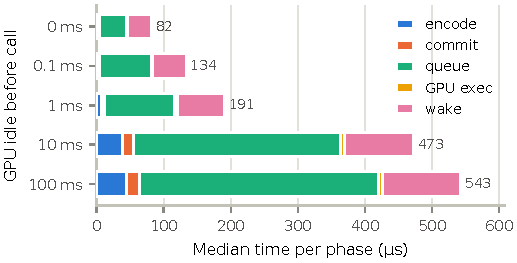
\includegraphics[width=\columnwidth]{figures/round_trip.pdf}
  \caption{Empty-kernel round trip, broken down by phase, after the GPU has been idle for the given time
  (\texttt{waitUntilCompleted}). Phase medians, stacked. \claim{C3, C6}}
  \label{fig:roundtrip}
\end{figure}

\textbf{A round trip is mostly waiting.} An empty kernel (one thread, no memory access) costs
\RoundTripUsMin{}--\RoundTripUsMax{}\,\textmu s from encode to the CPU resuming; the absolute value varies between
sessions far more than within one. Encoding and commit account for \RoundTripCpuSharePctMin{}--\RoundTripCpuSharePctMax{}\%.
The rest is queueing (\RoundTripQueueUsMin{}--\RoundTripQueueUsMax{}\,\textmu s) and wake-up
(\RoundTripWakeUsMin{}--\RoundTripWakeUsMax{}\,\textmu s) \claim{C3}. So a faster
submission API cannot remove this cost.

\textbf{Batching: command buffers, not dispatches.} An extra dispatch in an encoder adds \PerDispatchUs{}\,\textmu s;
an extra command buffer adds \PerCommandBufferUsMin{}--\PerCommandBufferUsMax{}\,\textmu s,
\CbOverDispatchMin{}--\CbOverDispatchMax{}$\times$ more \claim{C4}.

\textbf{Waiting.} Busy-polling an \texttt{MTLSharedEvent} still observes completion no sooner than
\SpinWakeFloorUs{}\,\textmu s after \texttt{GPUEndTime} \claim{C5}, so the floor lies in the completion path rather than
in CPU thread wake-up. The four blocking methods add roughly 0--30\,\textmu s on top, and their ranking changed with
measurement order, so we do not rank them. Wake latency rises to a plateau of ${\sim}$100--110\,\textmu s once the GPU has
been busy for ${\gtrsim}$200\,\textmu s. It does so equally after read-only and write-heavy kernels \claim{C16},
which rules out dirty-cache write-back as the main cause. \todo{mechanism: power-state hypothesis; Instruments trace}

\textbf{Idleness is expensive.} After the GPU has been idle for 100\,ms, the same empty round trip is
\IdleHundredMsRatioMin{}--\IdleHundredMsRatioMax{}$\times$ slower than back to back
(\IdleHundredMsUsMin{}--\IdleHundredMsUsMax{} vs.\ \IdleZeroUsMin{}--\IdleZeroUsMax{}\,\textmu s), mostly as queueing,
and CPU-side encode also slows (Fig.~\ref{fig:roundtrip}) \claim{C6}. Back-to-back benchmarks, including our own
crossover measurements, therefore understate what sporadic GPU use costs an application.

% ---------------------------------------------------------------------------
\section{Memory: setup, not bandwidth}\label{sec:memory}

\begin{figure}[t]
  \centering
  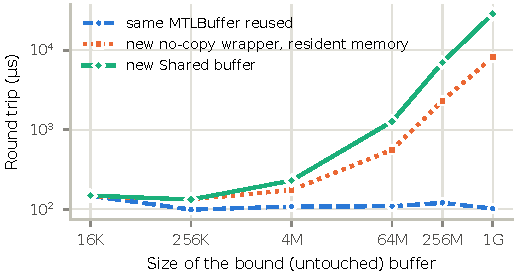
\includegraphics[width=\columnwidth]{figures/first_use.pdf}
  \caption{First GPU use of a buffer the kernel never touches. A new no-copy wrapper over memory that is already
  resident (``rewrap'') costs almost as much as new memory; reusing the same \texttt{MTLBuffer} does not.
  \claim{C7}}
  \label{fig:firstuse}
\end{figure}

\textbf{Storage mode does not change bandwidth.} GPU read and write bandwidth for Shared, Private and no-copy buffers
differ from their mean by at most \StorageModeMaxDevPctMax{}\% at 64--256\,MiB \claim{C8}.

\textbf{Each new buffer object pays a mapping cost.} Creating an \texttt{MTLBuffer} takes microseconds, because
backing is lazy. Its \emph{first GPU use} is what costs: a one-thread kernel that binds but never touches the
buffer. Wrapping already-resident host memory in a new no-copy buffer costs
\RewrapSixtyFourMUsMin{}--\RewrapSixtyFourMUsMax{}\,\textmu s at 64\,MiB and \RewrapOneGMsMin{}--\RewrapOneGMsMax{}\,ms at
1\,GiB, against \ReusedOneGUsMin{}--\ReusedOneGUsMax{}\,\textmu s when the same buffer object is reused
(Fig.~\ref{fig:firstuse}) \claim{C7}. A runtime that wraps tensors per call, as our own matmul did, pays this every
call. It accounts for roughly half of the queueing growth we saw in GEMM at $2048^2$--$4096^2$. Beischl et
al.~\cite{beischl2026damon} found the underlying mechanism on an M4 Pro: at the first kernel launch, each
\emph{newly allocated} shared buffer is wired (10--60\,GB/s) and then made coherent (70--120\,GB/s), and allocating
memory once avoids both. Our fresh-buffer and rewrap rates (${\approx}$38 and ${\approx}$120--130\,GB/s at 1\,GiB)
match those two passes. What we add is that the coherence pass recurs for every new buffer \emph{object}, even
over memory that is already resident and was never reallocated, so a runtime must cache the object, not only
the memory.
\todo{replace ``roughly half'' with the measured fraction once M7 caches wrappers}

\textbf{Large GPU-written buffers are slower to write.} Writing 1\,GiB as one buffer reaches \WriteOneBufferGBs{}\,GB/s;
the same bytes as 256\,MiB buffers reach \WriteChunksGBs{}\,GB/s \claim{C15}. A second pass is no faster, so this is not
first-touch. \todo{mechanism: GPU address-translation reach is the leading hypothesis}

\textbf{A new Shared buffer is slow for two passes.} CPU writes into a just-created Shared buffer run at
\FreshWriteOneGBs{}, then \FreshWriteTwoGBs{}, then \FreshWriteFourGBs{}\,GB/s, which matches host memory
\claim{C14}. Measurements that time the second pass (as our first characterization did) wrongly conclude that
Shared memory is slow.

% ---------------------------------------------------------------------------
\section{Interaction and heat}\label{sec:interaction}

\textbf{No cross-device eviction, but costly handoff.} After the GPU streams 16--256\,MiB of \emph{other} memory, a
sequential CPU pass over its own 1--12\,MiB working set, which fits in the performance cluster's L2, changes little
relative to the tiny-GPU control: the worst of 18 cells per session is \NoEvictMaxAbsPctMin{}--\NoEvictMaxAbsPctMax{}\% \claim{C9}. Our pre-registered bound was 10\%,
and one cell exceeded it in one session, so we report this claim as \emph{\verdictof{C9}} rather than established.
\todo{update wording once more sessions are in} When the GPU has written the CPU's own data, the next CPU pass is
\HandoffMinPctMin{}--\HandoffMaxPctMax{}\% slower \claim{C10}: the cost of a GPU$\rightarrow$CPU handoff, not of GPU
traffic as such. This is consistent with Alpay and Ba\c{s}aran~\cite{residualcache}, who find a 31--63\% slower first
CPU pass after a 64--512\,MiB GPU footprint on an M4 Pro. Their probe touches unrelated memory with an 8\,KiB stride
chosen to reside in the system-level cache shared with the GPU, and their contiguous-line control shows almost no
effect. GPU traffic therefore displaces SLC-resident CPU data, not a sequential working set held in the CPU's L2.
Their idle control waits with \texttt{waitUntilCompleted}, so it does not hold CPU clocks constant across GPU passes
of different length, as our spinning controls do. \todo{their SLC probe is now in cache\_interference
(pre-registered as C17: ${\geq}$15\% after a 256\,MiB GPU write vs.\ the tiny control); report once sessions include it} Running both at once is expensive: while the
GPU streams writes, CPU work slows by a median of \ConcurrentMedianPctMin{}--\ConcurrentMedianPctMax{}\% \claim{C11}, which argues against offloading
to the GPU merely to ``free'' the CPU.

\begin{figure}[t]
  \centering
  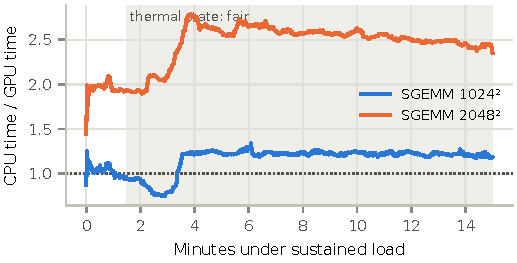
\includegraphics[width=\columnwidth]{figures/thermal.pdf}
  \caption{CPU time / GPU time for SGEMM under 15\,min of sustained mixed load (30\,s rolling median). Values above
  1 mean the GPU is faster. macOS reported thermal state \emph{fair} from 1.5\,min onward. \claim{C13}}
  \label{fig:thermal}
\end{figure}

\textbf{The crossover drifts, invisibly.} With pre-allocated outputs on both sides, Accelerate beats MPS clearly at
$128^2$ (CPU/GPU time \CrossRatioSmallMin{}--\CrossRatioSmallMax{}) and narrowly at $1024^2$
(\CrossRatioOneKMin{}--\CrossRatioOneKMax{}); the GPU wins at $2048^2$ (\CrossRatioTwoKMin{}--\CrossRatioTwoKMax{})
\claim{C1}. The crossover therefore lies between $1024^2$ and $2048^2$ on a cool machine. Under 15 minutes of mixed CPU+GPU load, CPU throughput falls by \ThermalCpuLossPct{}\%
and GPU throughput by \ThermalGpuLossPct{}\% \claim{C12}. The $1024^2$ ratio moves from \DriftRatioStart{} to
\DriftRatioEnd{}, making the GPU the better choice (Fig.~\ref{fig:thermal}) \claim{C13}. The largest step occurs
while macOS reports the same thermal state throughout, so \texttt{NSProcessInfo.thermalState} is too coarse to
guide placement. The thermal results so far rest on a single valid run (C13: \verdictof{C13}): a second run was excluded because the
power adapter was disconnected and a video call ran during it (both visible in the system power log), and the
benchmark now stops itself if the power source changes. \todo{report per heater load (cpu / gpu / mixed) once
sessions cover all three}

% ---------------------------------------------------------------------------
\section{Implications for runtimes}

\begin{itemize}
  \item \emph{Batch into command buffers}, not just dispatches; a command buffer costs ${\sim}$\CbOverDispatch{}$\times$ a dispatch.
  \item \emph{Keep \texttt{MTLBuffer} objects alive} with their memory. Re-wrapping resident memory is not free, so a no-copy
        wrapper should be cached alongside the tensor storage.
  \item \emph{Model idleness}: the cost of the next GPU call depends on how long the GPU has been idle.
  \item \emph{Split very large GPU-written buffers} (${\leq}$256--384\,MiB per buffer on this machine).
  \item \emph{Place work using measured, recent performance}, not static size thresholds or the OS thermal state;
        price GPU$\rightarrow$CPU handoffs and concurrency, not just kernel time.
\end{itemize}
\todo{check each against MLX's allocator (buffer cache, residency sets) and say which MLX already does}

% ---------------------------------------------------------------------------
\section{Related work}

Hübner et al.~\cite{huebner2025apple} and Kenyon and Capano~\cite{kenyon2022apple} characterize M-series throughput,
bandwidth and energy for HPC kernels. Feng et al.~\cite{feng2025profiling} attribute part of the training gap to kernel
launch time and page faults; we measure those costs directly. Beischl et al.~\cite{beischl2026damon} identify wiring and
coherence passes on newly allocated Metal shared buffers and amortize them in a database system
(\S\ref{sec:memory}). Alpay and Ba\c{s}aran~\cite{residualcache} measure residual SLC displacement after completed
GPU work (\S\ref{sec:interaction}). FusionML~\cite{fusionml} splits prefill matmuls across MLX's CPU and GPU streams
and shows that MLX's lazy graph serializes cross-stream work unless inputs are materialized. On a fanless M1 its
speedups shrink under sustained load, and it reports a ${\sim}1.17\times$ GPU-side slowdown under co-execution;
we quantify the CPU side (\S\ref{sec:interaction}). None of these break down per-call fixed costs (queue, wake,
idle penalty) or track the CPU/GPU crossover over time. On other integrated and unified-memory
platforms, zero-copy has been shown not to be free~\cite{otterness2017jetson}, and CPU/GPU placement has been driven by
input size~\cite{qilin} and by online cost estimates~\cite{mnn,codl}. Our contribution is the per-phase fixed-cost breakdown and the idle penalty; the finding that the coherence pass
is per buffer \emph{object} rather than per allocation; the scoping of cross-device interference to handoff, SLC
residency and concurrency; and the crossover's drift under heat on a fanless device.

% ---------------------------------------------------------------------------
\section{Threats to validity}

One machine, one chip, one OS version; behaviour may differ on Pro/Max parts and later macOS. GPU timestamps come from
Metal and could carry driver-specific offsets; we verified their ordering against CPU timestamps but cannot see
inside the driver. Our own kernels are not tuned, so overhead claims use MPS or empty kernels. Thermal results depend
on ambient temperature, which we do not control. \todo{record room temperature per session}

% ---------------------------------------------------------------------------
\section{Conclusion}

On a fanless M4, the cost of using the GPU is dominated by fixed costs that unified memory does not remove: queueing,
completion signalling, idle wake-up and per-buffer-object setup. Its value relative to the CPU also shifts under heat.
Runtimes that cache buffer objects, batch command buffers and place work from measured recent cost can recover
much of this. ComputeEdge, its probes and all raw data are available at \todo{URL / archive DOI}.

\bibliographystyle{IEEEtran}
\bibliography{refs}

\end{document}
